\documentclass[11pt]{article}

\usepackage[letterpaper,margin=0.75in]{geometry}
\usepackage{booktabs}
\usepackage{graphicx}
\usepackage{listings}
\usepackage{mathtools}
\usepackage{underscore}

\setlength{\parindent}{1.4em}

\begin{document}

\lstset{
  language=Python,
  basicstyle=\small,          % print whole listing small
  keywordstyle=\bfseries,
  identifierstyle=,           % nothing happens
  commentstyle=,              % white comments
  stringstyle=\ttfamily,      % typewriter type for strings
  showstringspaces=false,     % no special string spaces
  numbers=left,
  numberstyle=\tiny,
  numbersep=5pt,
  frame=tb,
}

\title{Congestion Control Part 1}

\author{Nathan Davis}

\date{Mar 14, 2016}

\maketitle

\section{Setup}

\subsection{General Setup}

The implementation for TCP and TCPPacket were initially copied from lab2. We won't cover any of the implementations from that lab and we'll assume that the beginning code base is taken from the result of that lab.

\subsection{Configuration Setup}

We added an option to transfer.py to allow the threshold (-t) to be set conveniently. The default is 100000.

\vspace{5mm}

\begin{lstlisting}
    parser.add_option("-t","--threshold",type="int",dest="threshold",
                      default=100000,
                      help="beginning threshold for tcp")
\end{lstlisting}

\vspace{5mm}

This threshold is passed in to TCP using the constructor and set as a class variable.

\vspace{5mm}

\begin{lstlisting}
    c1 = TCP(t1,n1.get_address('n2'),1,n2.get_address('n1'),1,a,
        window=self.window,threshold=self.threshold)
\end{lstlisting}

\vspace{5mm}

\subsection{Network Setup}

For the networks in this paper, we set up two nodes. We used the same structure for each part and varied the threshold size. The configuration looks like this:

\vspace{5mm}

\begin{lstlisting}
    # n1 -- n2
    #
    n1 n2
    n2 n1

    # link configuration
    n1 n2 0.8Mbps 100ms
    n2 n1 0.8Mbps 100ms
\end{lstlisting}

\vspace{5mm}

\section{TCP Tahoe}

\subsection{Slow Start}

Whenever TCP Tahoe receives an ACK, it increases the window size. There are two ways in which it does this, either by the slow start method or additive increase. We used a variable to keep track of the different ways TCP should increase window size. We called this variable the state.

\vspace{5mm}

\begin{lstlisting}
    # State determines slow start vs. additive increase
    # 0 = slow start
    # 1 = additive increase
    self.state = 0
\end{lstlisting}

\vspace{5mm}

When using the slow start method, TCP increases the window size by the number of bytes sent. This causes the growth to be exponential. Effectively, two new packets are sent out for every ACK received. If the window grows to equal or greater than the size of the threshold, slow start is halted and additive increase is used instead.

\vspace{5mm}

\begin{lstlisting}
    # Increase the window
    if self.state == 0:
        # Slow Start
        self.window += packet.ack_packet_length
        # If the window equals or exceeds the threshold, stop slow start
        if self.window >= self.threshold:
            self.state = 1
\end{lstlisting}

\vspace{5mm}

In order to increase the window size by the length of the packet, we added that information to the ACK packets. When the receiver sends an ACK it recordes the size of the original packet in the ACK.

\vspace{5mm}

\begin{lstlisting}
    self.send_ack(packet.sent_time, packet.length)
\end{lstlisting}

\vspace{5mm}

In the end, we see an exponential increase in the number of packets sent in the window. The following sequence diagram has a threshold of 100,000 bytes and the file is fairly small. The slow start remains in effect throughout the entire transmission.

\vspace{5mm}

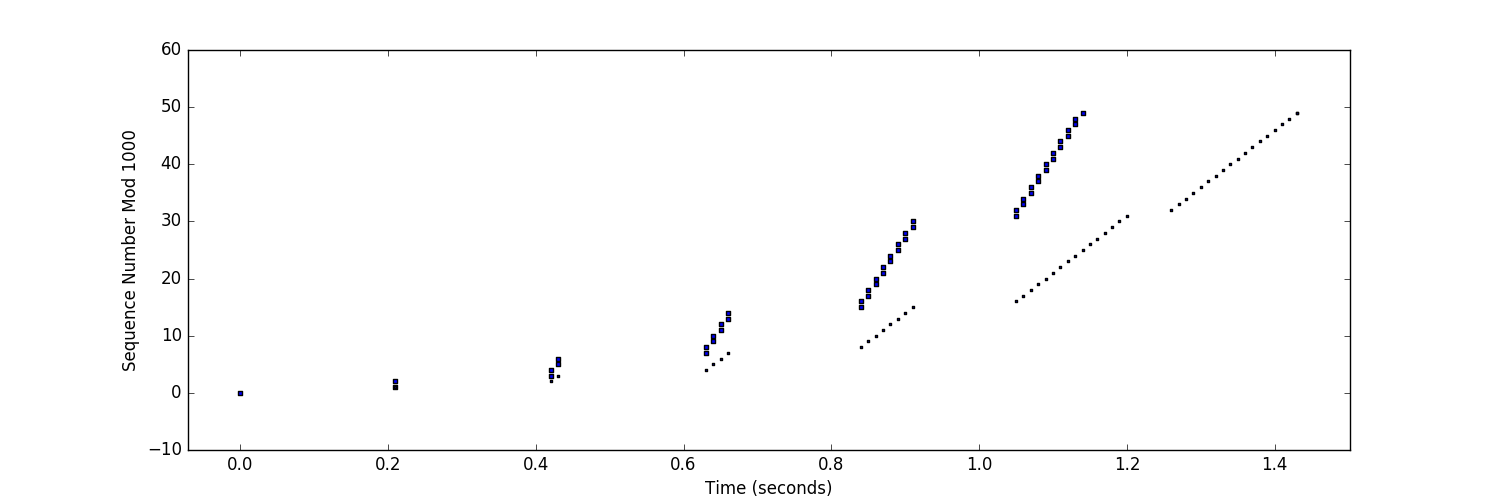
\includegraphics[width=17cm]{charts/slowstart.png}

\vspace{5mm}

The graph shows that growth is exponential. Each time packets are sent, the number of packets sent doubles. Since slow start continues through the entire transmission of the file, we only see slow start at work here.

\subsection{Additive Increase}

Additive increase adds a semi-static number to the window size. This number is determined with the following equation.

\vspace{5mm}
\(Increase = \frac{MSS \times Number of Bytes Acknowledged}{Window Size}\)
\vspace{5mm}

This is used so that as the window size grows, the added window size will tend to grow smaller. As the window size approaches infinity, the increase will approach zero. The increase size is also dependent on the size of the packet that was ACKed.\par

Additive increase is marked with the state variable. When state is equal to 1, we use additive increase to change the window size.

\vspace{5mm}

\begin{lstlisting}
    elif self.state == 1:
        #Additive increase
        increment = self.mss * packet.ack_packet_length / self.window
        self.window += increment
\end{lstlisting}

\vspace{5mm}

In the following experiment we set the threshold to 16000 so that additivie increase would kick in before the end of the file. We can see that after additive increase starts the window size increases at a rate much slower than exponential.

\vspace{5mm}

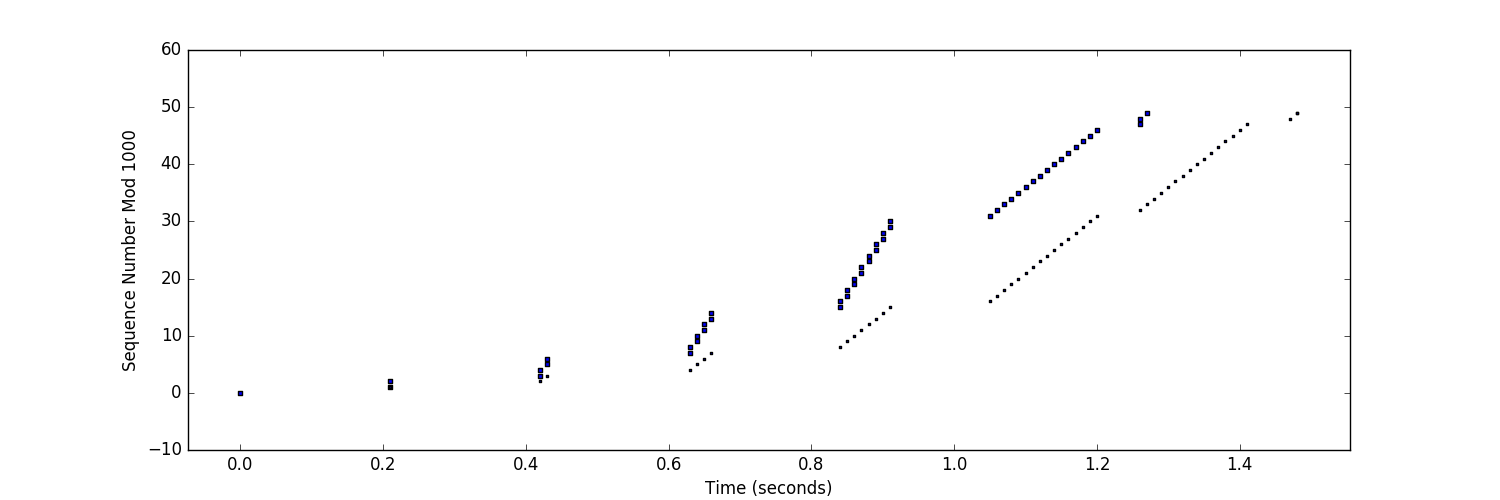
\includegraphics[width=17cm]{charts/additiveincrease.png}

\vspace{5mm}

\subsection{Fast Retransmit}

When three duplicate ACKs are detected, we need to immediately retransmit that packet. In order to track when duplicate ACKs are received, we use two variables, one to keep track of the last ACK number and one to keep track of how many times we've seen it.

\vspace{5mm}

\begin{lstlisting}
    # Most recent ack (used for calculating three duplicate acks)
    self.last_ack = None
    # Same ack count (used for calculating three duplicate acks)
    self.same_ack_count = 0
\end{lstlisting}

\vspace{5mm}

When we receive an ACK, we check if it's the same as the last one we received. If the ACK number is different from the ACK received before that we set the last ACK to that packet's ACK number and set the count to 1. We also proceed to process the ACK as normal. We increase the window size, slide the received window and send packets according to the new window size.

\vspace{5mm}

\begin{lstlisting}
    # Watch for three duplicate acks
    if self.last_ack != packet.ack_number:
        # If a new ack is received
        self.last_ack = packet.ack_number
        self.same_ack_count = 1
        self.increaseWindow(packet)
        self.slideWindow(packet)
        self.sendNextBatch()
\end{lstlisting}

\vspace{5mm}

If the ACK is the same number as the previous ACK, we increase the count.

\vspace{5mm}

\begin{lstlisting}
    else:
        # A duplicate ack has been received
        self.same_ack_count += 1
\end{lstlisting}

\vspace{5mm}

We also check to see if that ACK number has been seen more than three times. If this occurs, we reset the ACK count, set the threshold to half the window size, and retransmit. The retransmit will send the next packet and trigger slow start again.

\vspace{5mm}

\begin{lstlisting}
    if self.same_ack_count > 3:
        # When the fourth ack with the same number is received (3 duplicates)
        self.trace("Three duplicate ACKs. Ignoring duplicate ACKs for same sequence number")
        self.same_ack_count = -100
        self.threshold = max(self.window/2, self.mss)
        self.trace("Set new threshold to %d" % self.threshold)
        self.cancel_timer()
        self.retransmit({},duplicate_acks=True)
\end{lstlisting}

\vspace{5mm}

\subsection{AIMD}

Anytime a retransmit is triggered, we also trigger a slow start. Because of this, we see the pattern of additive increase and multiplicative decrease. In the following experiment we manually dropped packet 32. To manually drop packets, we added an attribute to the packet to mark it. We manually count the number of dropped packets to ensure we don't drop more than desired.

\vspace{5mm}

\begin{lstlisting}
    # Forced Loss, loss, AIMD dropped packets
    drop_list = [32000]
    if sequence in drop_list and self.dropped_count < len(drop_list):
        self.trace("Manually dropping packet %d" % sequence)
        packet.drop = True
\end{lstlisting}

\vspace{5mm}

When the packet is dropped, the window has grown to size 32000 bytes. The threshold is then set to half of the window size and slow start occurs until it reaches that new threshold. Afterwards, additive increase continues as normal.

\vspace{5mm}

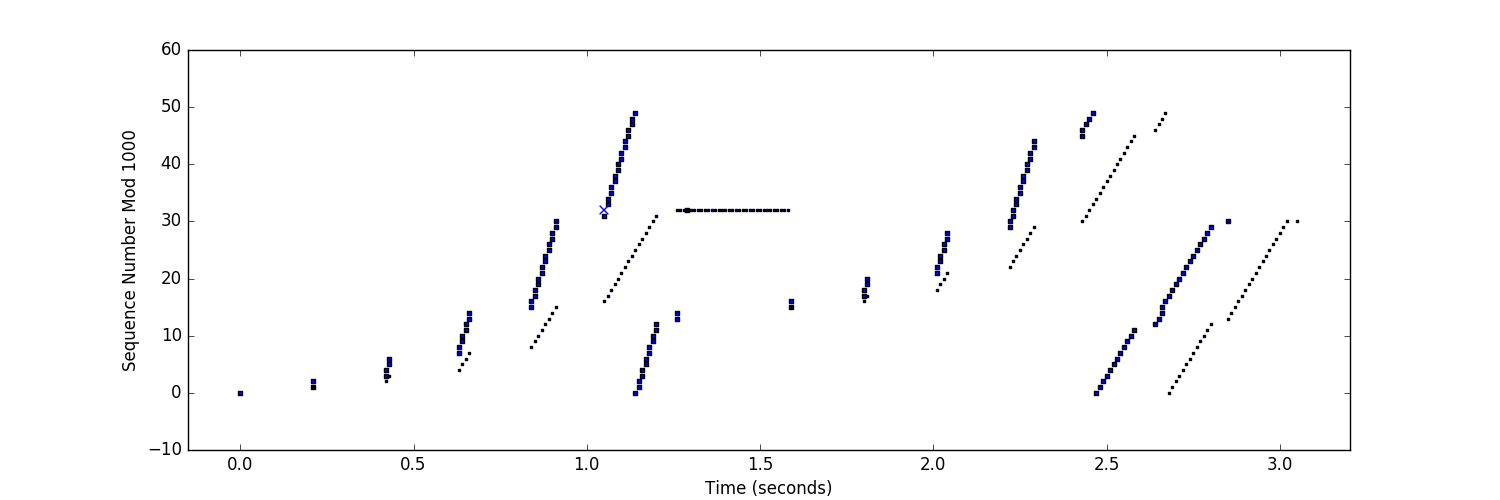
\includegraphics[width=17cm]{charts/aimd.png}

\vspace{5mm}

We can see the dropped packet around 1.1 seconds and the immediate retransmission after three duplicate ACKs at around 1.3 seconds. The transmission then proceeds with slow start up to half of the previous window size and then initiates additive increase.

\subsection{Burst Loss}

When there are multiple packets lost in rapid succession, we can see that the Tahoe will still recover with a slow start from 1 MSS. For burst loss we have to manually put in the packets to drop.

\vspace{5mm}

\begin{lstlisting}
    drop_list = [32000, 33000, 34000] # For burst loss
\end{lstlisting}

\vspace{5mm}

Here's the results we get:

\vspace{5mm}

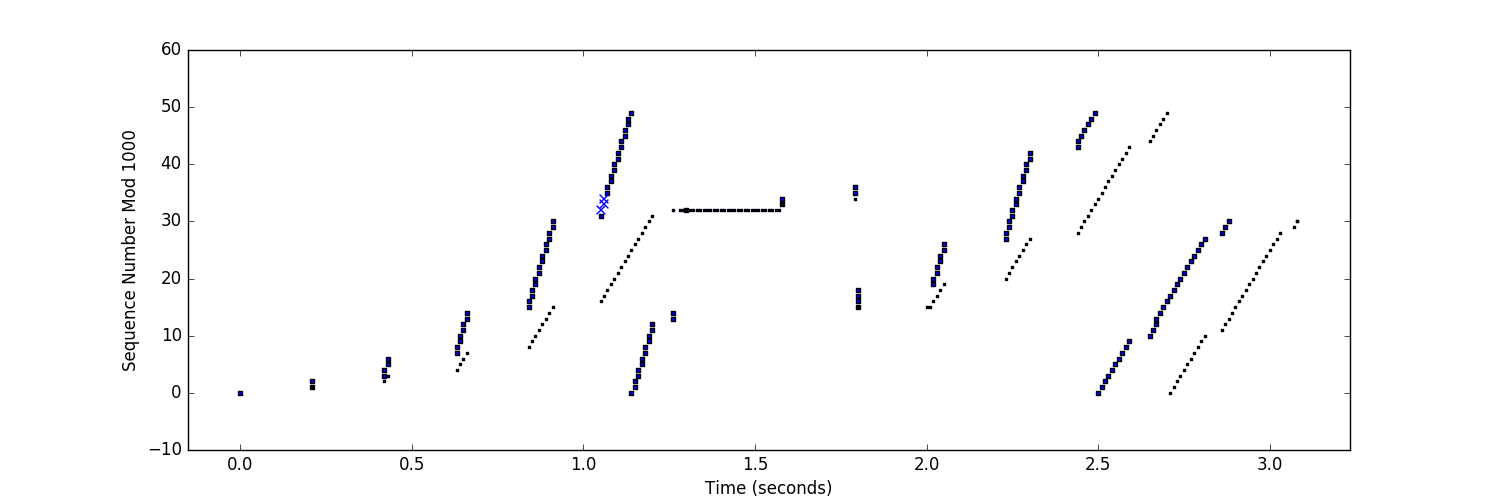
\includegraphics[width=17cm]{charts/burstloss.png}

\vspace{5mm}

From the chart above we can see that many packets sent after the lost packets send back ACKs for the original lost packet. However, after the lost packets are resent, the receiver immediately "catches up" to where it had left off. Shortly afterwards, it reaches the new threshold and begins additive increase.

\section{Fast Recovery (Reno)}

For the script included, we used -r to signify that fast recovery should be used.

\vspace{5mm}

\begin{lstlisting}
    parser.add_option("-r","--fast-recovery",dest="fast_recovery",
                      default=False, action="store_true",
                      help="use fast recovery (reno)")
\end{lstlisting}

\vspace{5mm}

When implementing fast recovery, everything stays the same except for the recovery after a loss caused by three duplicate acks. In this case, a retransmission occurs as normal, and the window is set to half of the current window size. From there, additive increase continues as normal. 

\vspace{5mm}

\begin{lstlisting}
    def slow_start(self, duplicate_acks=False):
        if duplicate_acks and self.fast_recovery:
            # If using fast recovery and three duplicate acks are detected,
            # set the window to half the original and 
            # keep going with additive increase
            self.window = int(round(self.window/2 / self.mss) * self.mss)
            self.state = 1
        else:
            # Otherwise reset the window to 1 mss and use slow start
            self.window = self.mss
            self.state = 0
\end{lstlisting}

\vspace{5mm}

In optimal conditions where only one loss occurs occasionally, this can be a great benefit. In the diagram below, we see that one packet was dropped and retransmitted when multiple ACKs were received. However, the window doesn't drop all the way back down to 1 MSS. Instead, it continues from half of its previous window size.

\vspace{5mm}

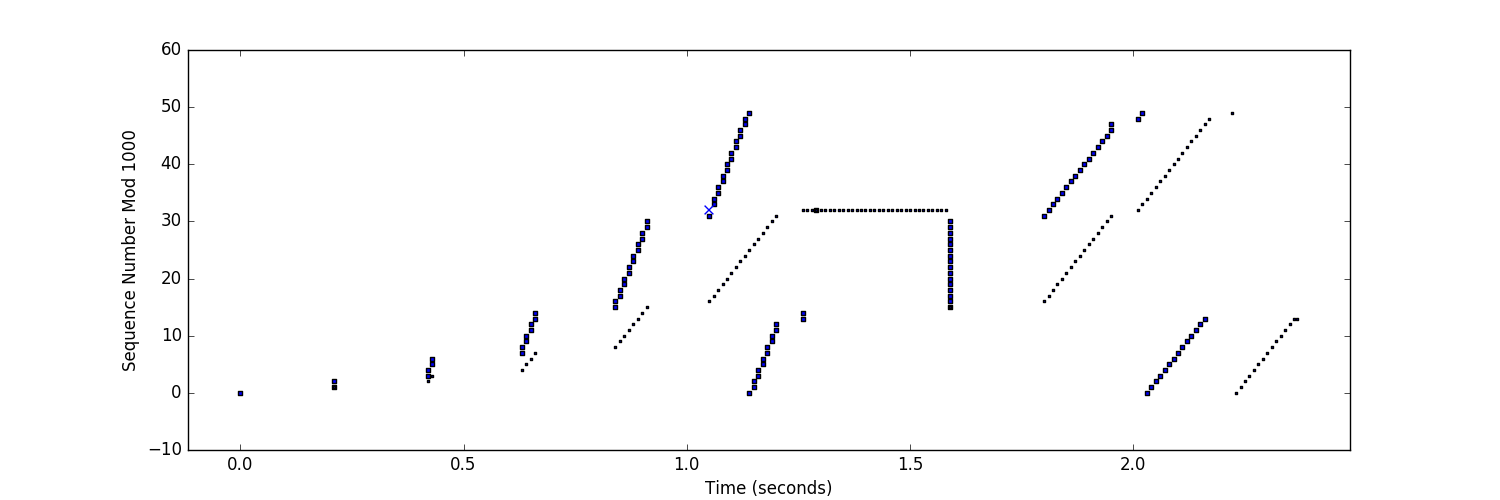
\includegraphics[width=17cm]{charts/renosingle.png}

\vspace{5mm}

However, we can see that Reno reacts very poorly to burst loss in the chart below.

\vspace{5mm}

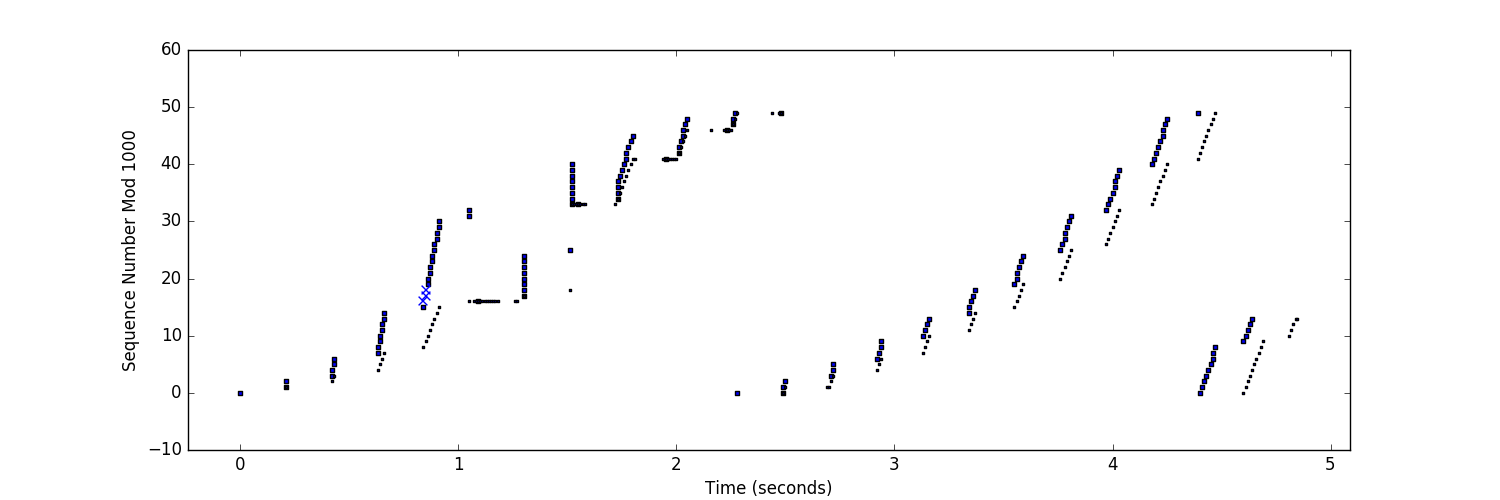
\includegraphics[width=17cm]{charts/renoburst.png}

\vspace{5mm}

After the original packet loss, our implementation of Reno resends the missing packet but fails to resend the next two immediately. When the missing packet gets through, it continues to send packets at a rate of half the previous window size. The first two packets fill in the missing spots in the receiver's buffer but the rest of the packets aren't needed and so another set of duplicate ACKs is generated. Because of those duplicates, the send buffer is once again reset and a full duplicate window of packets is sent. This continues for a few rounds until Reno gets to a small enough window where it resets itself.

\vspace{5mm}

Note: Our chart does not look the same as the one in the SACK paper because our buffer resets when it sends data thus nulling out the number of outstanding packets and restarting from the last ACK received. Notwithstanding the fact that it doesn't yield the exact same results, the staggering number of duplicate packets sent in this last experiment is educational in itself.

\vspace{5mm}

\vspace{5mm}

\end{document}
